\chapter{Topological manifolds}

\section{Some point set topology}

Some (set theoretical) conventions for the whole course:
\begin{itemize}
    \item \(A\subset B\) means A subset (not necessarily proper!) of B, i.e. \(\subset =\subseteq\)
    \item A \highlight{neighborhood} of some point \(p\in X\) means \textit{an open set \(U\subset X\) containing \(p\)}
    \item Given \(p=(p_1,\dots,p_n)\in\R^n,r>0\), \(B_r^n(p)\coloneqq \{(x_1,\dots,x_n)\mid \sum_{x_i-p_i}^2<r^2\}\). Often while \(B_s=B_s^n(0)\subset\R^n\)
\end{itemize}

\subsection{Locally Euclidean spaces}

\begin{definition*}
    A topological space \(X\) is called \dhighlight{locally Euclidean of dimension \(n\geq 0\)}, if every 
    point of \(X\) is contained in a neighborhood homeomorphic to some open subset of $\R^n$. 
\end{definition*}

\begin{remark}
    When we speak of a topological space as being \highlight{locally Euclidean}. The dimension is fixed and implicit.
\end{remark}

\begin{definition*}
    Assume that \(X\) is locally Euclidean. A \dhighlight{chart} is a pair \(U,\phi\), where \(U\subset X\),
    \(\phi:U\to\R^n\) is a homeomorphism into its image. Given \(p\in X\), we say that \(U,\phi\) is 
    \dhighlight{centered at \(p\)} if \(p\in U\) and \(\phi(p)=0\in\R^n\)
    \begin{figure}[H]
        \centering
        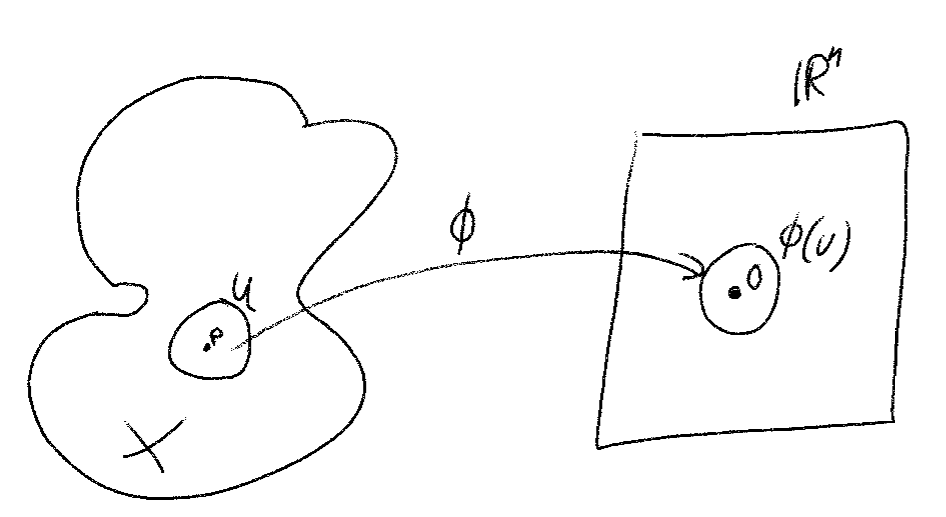
\includegraphics[width=.7\textwidth]{sketch_1_01.png}
        \caption{Sketch 1.01}
    \end{figure}
\end{definition*}

\begin{lemma}\label{lem:1.1}
    The following are equivalent (TFAE):
    \begin{itemize}
        \item \(X\) is locally Euclidean
        \item For any \(p\in X\), there is a chart \(U,\phi\) centered at \(p\) with image \(\phi(U)=B_1\)
        \item For any \(p\in X\), there is a chart \(U,\phi\) centered at \(p\) with image \(\phi(U)=\R^n\)
    \end{itemize}
\end{lemma}

\begin{proof}
    2. and 3. are equivalent, since \(B_1 \simeq \R^n\) are homeomorphic (\(B_1^n\ni x\mapsto \frac{x}{1-\Vert x\Vert}\)) % TODO: FIX 
    
    2. \(\implies \) 1. is tautological

    1. \(\implies\) 2. given \(p\in X\), since \(X\) is locally Euclidean, there exists \highlight{some} chart \(U,\phi\), \(p\in U\).
    \(psi:U\to\R^n\), homeo onto its image \(psi(U)=O\subset\R^n\). By translativity \(\R^n\ni x\mapsto x-\psi(p)\), one can assume 
    \(\psi(p)=0\in\R^n\). By scaling \(\R^n (x\mapsto \lambda x,\lambda>0)\), can assume \(B_1\subset\psi(U)\).
    Let \(U'=\psi^{-1}(B_1)\), then \((U,\psi)\) as claimed. 
\end{proof}

\subsection{Hausdorff spaces}

\begin{definition*}
    A topological space \(X\) is called Hausdorff, if given any \(p_1\neq p_2\),\(p_1,p_2\in X\), there exist neighborhoods \(p_1\in U_1,p_2\in U_2\) s.t. \(U_1\cap U_2=\emptyset\).
    \begin{figure}[H]
        \centering
        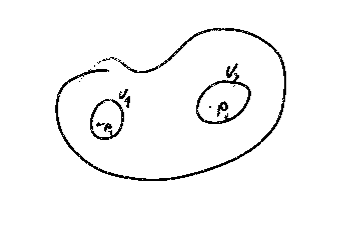
\includegraphics[width=.7\textwidth]{sketch_1_02.png}
        \caption{Sketch 1.02}
    \end{figure}
\end{definition*}

\begin{example}
    \begin{itemize}
        \item \(\R^n\)
        \item CW complexes
        \item most reasonable spaces
    \end{itemize}
\end{example}

\begin{example}[Not Hausdorff]
    \(X=\{0,1\}\), open subsets \(\emptyset,\{0\},\{0,1\}\)
\end{example}

\begin{remark}
    \(X\) is homeomorphic to \(\R/\R^*\) (quotient topology), \(R^*, (s,x\mapsto sx)\)
\end{remark}


\begin{lemma}\label{lem:1.2}
    Let \(X\) be Hausdorff. 
    \begin{enumerate}
        \item[(a)] point sets \(\{x\}\) are closed
        \item[(b)] convergent sequences have unique limits. (\(x_n\to p,x_n\to q\implies p=q\)) 
        \item[(c)] compact sets are closed 
    \end{enumerate}
\end{lemma}

\begin{proof}
    (c) \(\implies \) (a)

    For (c): Let \(K\subset X\) be compact. Want to show \(K^c\) is open. Pick \(p\in K^c\). For each 
    \(q\in K\), we can choose \(U_q\ni q, U_p\ni p: U_q\cap U_p=\emptyset\) Since K is compact, it can be covered by \(U_{q_1},\dots,U_{q_l}\). Then \(\bigcap_{i=1}^l U_{q_i}\) is oen and contains 
    \(p\), disjoint, then \(\bigcup_{i=1}^l U_{q_i}\supset K\).

    \begin{figure}[H]
        \centering
        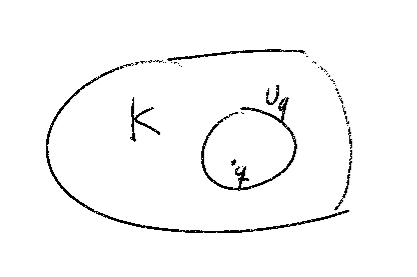
\includegraphics[width=.7\textwidth]{sketch_1_03.png}
        \caption{Sketch 1.03}
    \end{figure}

    (b) Suppose for contradiction that \(x_i\to p,x_i\to q\) and \(p\neq q\). Since \(X\) is Hausdorff, \(\exists U\ni p, O\ni q, U\cap O=\emptyset\). But for \(N>>0 x_i\in U, x_i\in O\forall i>N\)
\end{proof}


\section{Basis and covers}

Let \(X\) be a topological space.

\begin{definition*}
    A collection \(\cB\) of subsets of \(X\) is called a \dhighlight{basis(base)} for \(X\), if for any \(p\in X\)
    and any neighborhood \(U\ni p\), there exists an element \(\cU\in\cB\) s.t. \(p\in \cU\subset U\).
    \begin{figure}[H]
        \centering
        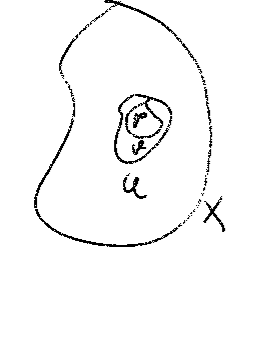
\includegraphics[width=.7\textwidth]{sketch_1_04.png}
        \caption{Sketch 1.04}
    \end{figure}
\end{definition*}


\begin{lemma}\label{lem:1.3}
    \(\cB\) is a basis for \(X\iff\) every open set of \(X\) is a union of elements of \(\cB\).
\end{lemma}

\begin{proof}
    Trivial.
\end{proof}

\begin{definition*}
    A topological space \(X\) is \dhighlight{second-countable} if it admits a countable basis.
\end{definition*}

\begin{example}
    \begin{itemize}
        \item \(\R^n\), \(\cB=\{B_s^n(p)\mid s\in \Q_+,p=(p_1,\dots,p_n)\in\Q^n\subset \R^n\}\)
    \end{itemize}
\end{example}

\begin{lemma}\label{lem:1.4}
    The property of being second-countable is closed under 
    \begin{enumerate}
        \item[(a)] subspaces
        \item[(b)] finite unions
        \item[(c)] countable products
    \end{enumerate}
\end{lemma}

\begin{remark}
    The property of being second-countable is not closed under arbitrary quotients \(q:A\to A/B\). 
    An obvious sufficient conditions is for \(q\) to be an open map. (Since it is a pushforward)\marginnote{When constructing manifolds via quotients, check that it is still second-coutable!}
\end{remark}

\begin{lemma}\label{lem:1.5}
    If \(X\) is second countable, then any open cover of \(X\) admits a countable subcover.
\end{lemma}

\begin{proof}
    Let \(\cB\) be a countable basis for \(X\). Let \(\cC\) be an open cover. 
    Let \(\tilde{\cB}\subset\cB\) be the collection of basis elements \(U\), which are contained 
    in some \(\cU\in\cC\). Observe (key!) \(\tilde{\cB}\) is a cover of \(X\). For each \(U\in\tilde{\cB}\),
    choose \(\cU_U\in\cC\) such that \(U\subset \cU_U\). Then \(\{\cU_U\}\) is a countable subcover of \(\cC\).
\end{proof}

\begin{definition*}
    Let \(X\) be a topological space. An \dhighlight{exhaustion of \(X\) by compact subsets} is a sequence \(\{K_i\}_{i\in\N}\),
    where \(K_i\subset X\) compact and \(K_i\subset \interior(K_{i+1})\) and \(\bigcup_{i=1}^\infty K_i=X\).
\end{definition*}

Recall given \(A\subset X\). \(\interior(A)\coloneqq \{x\in A\mid x \text{ in a neighborhood } U\subset A\}\).


\begin{lemma}\label{lem:1.6}
    If \(X\) is locally Euclidean, Hausdorff and second countable. Then \(X\) admits an exhaustion by compact subsets.
\end{lemma}

\begin{proof}
    Since \(X\) is locally Euclidean, admits a basis \(\cB\) of open subsets having compact closure.\marginnote{That is take the close of \(B_{\frac{1}{2}}\subset\R^n\)}
    \begin{figure}[H]
        \centering
        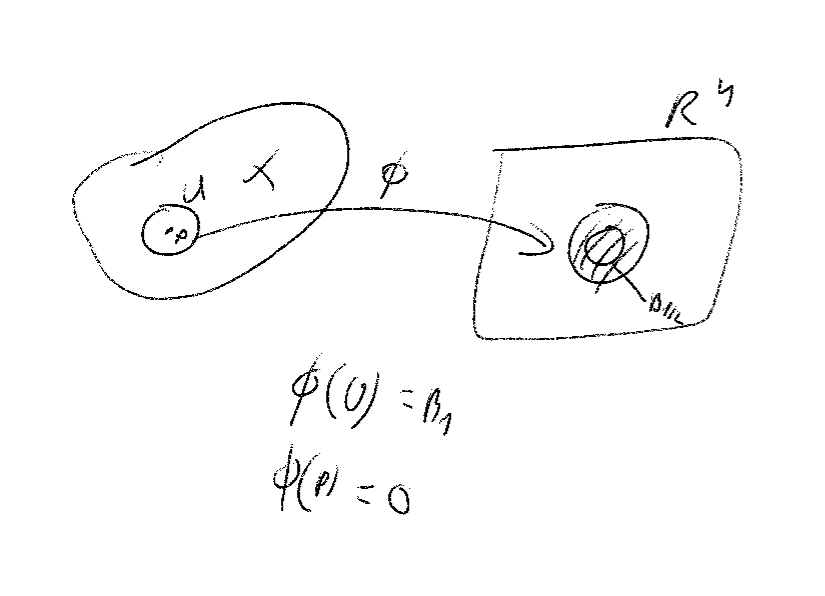
\includegraphics[width=.7\textwidth]{sketch_1_05.png}
        \caption{Sketch 1.05}
    \end{figure}
    By Lemma 1.5, one can extract a countable subcover \(\{U_i\}_{i=1}^\infty\). Set \(K_1=\overline{U_1}\).
    Assume that we already constructed \(K_1,\dots,K_k\) such that \(U_j\subset K_j\)
    and \(K_{j-1}\subset\interior(K_j),j\geq 2\). Since \(K_k\) is compact and \(K_k\subset X=\bigcup_{i=1}^\infty U_i\), then there exists some \(m_k\) such that 
    \(K_k\subset X=\bigcup_{i=1}^{m_k} U_i\) by compactness. Might as well assume that \(m_k\geq k\). Set 
    \[K_{k+1}=\overline{\bigcup_{i=1}^{m_k} U_i}=\bigcup_{i=1}^{m_k} \overline{U_i}.\] By construction \(K_{k+1}\) 
    is compact, \(K_k\subset \interior(K_{k+1})\). We get \(\{K_j\}_{j=1}^\infty\), \(U_j\subset K_j\) (because \(m_j\geq j\)) \(\implies \bigcup_{i=1}^\infty U_i=\bigcup_{i=1}^\infty K_i\)
\end{proof}




